\def\year{2015}
%File: formatting-instruction.tex
\documentclass[letterpaper]{article}
\usepackage{aaai}
\usepackage{times}
\usepackage{helvet}
\usepackage{courier}
\usepackage{graphicx}

\frenchspacing
\setlength{\pdfpagewidth}{8.5in}
\setlength{\pdfpageheight}{11in}
\pdfinfo{
/Title (Genkii - The Effects of Varying Sequential Rewards for User's Motivation to Complete a Set of Crowdfunded Tasks.)
/Author (Helmut Prendinger, Ruben Geraldes, Daniela Fontes, Daniel Morais, Rui Prada)
/Keywords (Crowdsourcing)}
\setcounter{secnumdepth}{2}  
\setlength\titlebox{8cm}
 \begin{document}
 
% The file aaai.sty is the style file for AAAI Press 
% proceedings, working notes, and technical reports.
%
\title{Genkii - An Affect Reporting Application for Studying the Effects of Fixed and Increasing Rewards}
\author{Ruben Geraldes \\
rubengeraldes@gmail.com \\
Instituto Superior T\'{e}cnico, \\ Universidade de Lisboa,\\
	Av. Prof. Cavaco Silva, \\ Taguspark Porto Salvo, Portugal\\ 
	\And Daniela Fontes\\
	daniela.fontes@ist.utl.pt \\
	Instituto Superior T\'{e}cnico, \\ Universidade de Lisboa,\\
	Av. Prof. Cavaco Silva, \\ Taguspark Porto Salvo, Portugal\\
	\AND Helmut Prendinger \\
	helmut@nii.ac.jp\\
	National Institute of Informatics,\\
	2-1-2 Hitotsubashi, Chiyoda-ku, \\ Tokyo, 101-8430, Japan \\ 
	\And Rui Prada\\
	rui.prada@tecnico.ulisboa.pt\\
	INESC-ID ,\\
	Av. Prof. Cavaco Silva, \\ Taguspark Porto Salvo, Portugal\\		
}



\maketitle

% If the title and author information does not fit in the area allocated,
% place \setlength\titlebox{height}
% after the \documentstyle line
% where {height} is something like 2.5in

\begin{abstract}

Genkii is a GPS enabled affective state reporting application. In this work we plan and execute a crowdsourced study using Yahoo Japan. Given a reward budget per user, we study the influence of offering a fixed reward in comparison to an increasing reward scheme. Even though the two methods perform very similarly, using an increasing reward scheme increases user completion of the set of tasks.

\end{abstract}

\section{Introduction}

\subsection{Motivation}



The ubiquity of hand-held devices opened up new opportunities for research. Nowadays it is accessible to perform off-site studies and collect data in real-time and across great geographical spans.

One of the ways to deploy these off-site studies is by using micro-tasks markets. We are specially interested in this type of crowdsourcing.

This new paradigm also gives rise to the search for new methodologies, and best practices, which may help the scientific community improve and stage new experiments, in a way that optimizes its resources.



Genkii was conceived after realizing some problems in attracting users for crowdsourced studies in Japan in previous test pilots and studies. The initial hypothesis for this problem in attracting users for social studies had to do with privacy issues.

We want to study the effects of varying inducements to get people to perform a determined task repeatedly.

\subsection{Outline}

\section{Related Work}
\subsection{Crowdsourcing}
\label{subsec:Crowdsourcing}

In order to set up a crowdsourcing campaign we use the framework suggested in \cite{Henze2013}.

\begin{enumerate}
		
\item Clearly identify the research goals; \item Select a study method; \item Devise an incentive mechanism;  \item Choose the target platform(s); \item Design and develop the mobile app; \item Prepare data collection; \item Implement a scheme to obtain informed consent from users; \item Distribute and promote the app; \item Continuously monitor data collection for a designated time period; \item Filter and analyze data to answer the research question
\end{enumerate} 
\cite{Henze2013}.


\subsection{Rewards and Motivation}



\begin{quote}
When explicit incentives seek to change behavior in areas like education, contributions to public goods, and forming habits, a potential conflict arises between
the direct extrinsic effect of the incentives and how these incentives can crowd
out intrinsic motivations in the run short and the long run.
\end{quote}
\cite{Gneezy2011}




The use of rewards to induce a desired behavior has been thoroughly studied. 
There has been a clear separation between intrinsic rewards and extrinsic rewards, and research points out that a high focus on incentives can ultimately lead to the alienation of creative thinkers. 
According to \cite{Gneezy2011}, there are instances where monetary rewards (extrinsic rewards), work well. Mechanical based, self-contained and well-specified tasks seem to be the primary candidates for the usage of extrinsic rewards to motivate, induce or boost the agent's performance\cite{Ariely2009}.

Crowdsourcing is often associated with Gamification, the use of game-design elements to achieve a more compelling user-experience driven by fun.


However there is criticism when using incentives in areas like education and forming habits, because they can hinder natural intrinsic motivation, and the dependence on rewards may lead to reward inflation, and lower the effort the agent is willing to put towards the task \cite{Irlenbusch2005}. 





\subsection{Crowdsourcing Platforms}


\subsubsection{Amazon's Mechanical Turk}

Amazon's Mechanical Turk is a platform which serves as an interface for the deployment of crowdsourced tasks that are considered easier for humans than machines. 

It creates a labor market in which individuals or corporations can list tasks (also known as HITs or “human intelligence tasks”), and a specified compensation. The workers can then elect to complete a determined task, against a deadline, and be compensated upon timely completion. The compensation for the worker is either being paid a determined amount, or a free volunteered work \cite{Mason2010}. 
This model has been referred to in the literature as a micro-tasks market\cite{Kittur2008}.

In \cite{Mason2010} it is shown and discussed the potential use of Amazon's Mechanical Turk for laboratory experiments for a low fee (between 0.01\$ and 0.10\$).
The main advantages cited for the merit of these studies are the convenience of the platform in reaching many users in a relatively short notice and it is mentioned that the average cost per user is very low, in the order of cents per task.
Also it has been shown \cite{Kittur2008} that, provided that the type of task is well-specified, easily measurable, and do not put a lot of emphasis on creativity,  the quality of work performed on Amazon's Mechanical Turk is as good, and maybe even better than, work performed by experts paid under traditional contracting arrangements.

Further experiment design recommendations offered in \cite{Kittur2008} including the concern in devising the tasks such that it discourages random or malicious completion, by making a good performance require the same or less effort than a tampered one.


\subsubsection{Yahoo Crowdsourcing Japan}

Yahoo Crowdsourcing Japan works in a similar way as the Amazon's Mechanical Turk. 


\section{Genkii}


Genkii is an application that enables gps localized satisfaction reports. Users report their ''Genkiiness'', by performing three different gestures:

\begin{itemize}
	\item Circle meaning that the person feels happy/genkii;
	\item Triangle which represents an ''OK'' state;
	\item Cross which denotes sadness.
\end{itemize}





\subsection{Implementation}
\label{subsec:implementation}



\subsection{Crowdsourcing Campaign}



Following the methodology suggested by \cite{Choi2014}, we want to perform a study where one group will be considered our baseline by receiving a fixed reward for each task over time.
Besides our control group, we devise a second incentive scheme, that using the same amount of points, poses as a progressive reward system. We can compare both reward schemes on \ref{tab:rewards}.

Our goal is to study this and compare these two incentive schemes, specially by studying user enrollment rates and user drop rates.

\begin{table}[!h]
	\caption{ Scheme of rewards used for the crowdsourcing campaign. Using the same amount of reward points, for our first group these rewards are the same for every task over time. On the second group, we devised an increasing reward mechanism. }
	\begin{center}
\begin{tabular}{|c|c|c|c|c|}
	\hline  Reward & Task 1  & Task 2  & Task 3  & Task 4 \\ 
	\hline  Stable Rewards & 20 & 20 & 20 & 20  \\ 
	\hline Increasing Rewards & 5 & 10 & 15 & 30  \\ 
	\hline 
\end{tabular} 

\begin{tabular}{|c|c|c|c|c|c|c|c|c|c|c|}
	\hline   Task 5 & Task 6 & Task 7 & Task 8 & Task 9 & Task 10 \\ 
	\hline   20 & 20 & 20 & 20 & 20 & 20 \\ 
	\hline   35 & 40 & 50 & 60 & 60 & 60 \\ 
	\hline 
\end{tabular} 
\end{center}
\label{tab:rewards}
\end{table}

As stated in Section \ref{subsec:Crowdsourcing}, we followed the framework proposed in \cite{Henze2013}.
\begin{enumerate}
	\item Our main research goal is to compare two different reward schemes using the same budget per user (fixed rewards versus increasing rewards), on a set of sequential tasks;
	\item We are going to compare user on-boarding and drop rates in order to understand how do the two rewards perform;
	\item By using Yahoo Crowdsourcing we award ''T-Points'', a popular loyalty points card;
	\item The target platform of the Genkii App is Android;
	\item We discuss the design of the application in detail on Section \ref{subsec:implementation} . We focused on creating a user interface using gestures, which makes the interaction with the application uncommon;
	\item Before launching the campaign featured in this study we performed several pilot tests, which enabled us to understand the Yahoo Crowdsourcing platform; 
	\item After the installation we present a tutorial where we explain the type of data collected, and the terms in which the data will be used;
	\item The Yahoo Crowdsourcing is an interesting solution to distribute our application, since it handles the promotion;
	\item During the campaign we monitor for the server uptime, ensuring the data is being properly retrieved;
	\item The last point has to to with filtering and answering the research question. In the following section we present and discuss the results obtained.
\end{enumerate}


The first campaign ran from 19/06/2015 to 26/06/2015. The second campaign featuring increasing rewards ran from 08/07/2015 to 15/07/2015.

%\subsection{Individual versus Group Analysis}
%
%One of the main concerns for the analysis of this experiment is whether to consider the aggregated group behavior or the individual behavior.
%
%After all our objective is to compare two reward schemes, and test our hypothesis. 
%
%** If we consider the group of users a system, then the aggregated behavior can be considered a legitimate approach, as we are interested on the overall behaviour of the system, when designing a large scale study. 
%
%An analogy is the way we study and understand temperature in Physics. Temperature is defined as a measure of the average kinetic energy of the particles in a system. We can define, derive, and predict an enormous range of behaviours, by measuring the temperature of the system. However the behaviour of an individual particle in the system, and its kinectic energy, is complex and difficult to associate with the behaviour of the group of particles.
%
%is a measure of the average kinetic energy of the particles in a system
%
%*theory of ergodicity

\subsection{Expectations and Hypotheses}

Intuitively we expect the fixed reward scheme to have a greater onboarding, with more players joining in enticed by a considerable reward. On the other hand, we expect fewer players joining the increasing reward version, but those who join will be motivated to get bigger and bigger rewards.

This experiment is going to be deployed in the Japanese population via Yahoo Crowdsourcing. Genkii, as a location-enabled mood reporting application, allows the capture of interesting information about its users. Even though there may be validity issues regarding the accuracy of Genkii to relay truthful reports, the system is designed in a way that the effort to report a false mood is exactly the same as for reporting the actual mood evaluated by the user, according to the best practices referred in \cite{Kittur2008}.

We hope we will be able to capture some insights about the people who use this service.

We also expect to collect a set of best practices, and lessons learned that can be applied to future crowdsourced studies, in particular, those using Yahoo Japan.  

%suggestion sentiment annalysis with Genkii
\section{Results}

The first campaign featuring a fixed reward scheme counted with 436 genkii reports.
115 users installed the Genkii application, and 79 users provided at least one report.

The main goal of this study is to compare the effect of rewards on the user's reporting behaviour.
At first glance in order to understand the data collected it's important to study the overall frequency of the user reports. In the Figure \ref{fig:freqreports1} we can observe that in fact there seems to be a considerable on-boarding effect with 39 users making 1 report. But we also have a group of 15 users that made more than the strictly required (10 reports).



As we can observe in Figure \ref{fig:freqreportsperday1} the campaign quickly took off. During the last three days, we verified a drop in the number of reports being made. Our hypothesis for this has to do with the architecture of the Yahoo crowdsourcing and a limit of times the each task could be unlocked, as we were primarily interested on studying the sequential behavior. Also, users understood that given the time constraint between reports (4 hours), it becomes more difficult to finish the set of 10 tasks.


The increasing reward campaign run from 08/07/2015 to 15/07/2015.
123 users installed the Genkii app during the campaign, with 94 users providing at least one report. We captured 623 Genkii reports during this campaign.

In both campaigns, we observe that the last four days see a drop in user acquisition. This may happen due the promotion placement made by Yahoo Crowdfunding. 

%This makes the second campaign 


\subsection{Reward Schemes}

In order to compare the two incentive schemes devised we use the user drop rate as a metric for how well the users stick with our 10 task program.

We verified that 9 users completed the 10 rewarded tasks during the fixed campaign reward. It is important to refer that in order to unlock a reward the reports have to be made with a 4-hour interval. There were 18 users who ended up making 10 or more reports, during the fixed reward campaign.

When using the increasing reward scheme we noted that 16 users finished the 10 rewarded tasks. Taking into account the user participation in the two campaigns, we can conclude that users on the increasing rewards scheme were more likely to finish the tasks (17\%) in comparison with the fixed rewards scheme where only 11.3\% of the users completed the 10 rewarded tasks.
In the increasing rewards campaign, 25.5\% of the users did more than 10 reports, in the fixed reward scheme 22.8\% did more than 10 reports.



Overall user participation decreases sharply during the first two quests, on both campaigns.
The most notorious difference between the two campaigns is the drop experiences between the first and second quest. 
The fixed reward scheme has an initial drop rate of 50\%. After the first reward, 35\% of the users did not claim any more rewards on the increasing reward incentive scheme.  
In the increasing reward scheme, the users have a smaller drop rate between the first and second quest, with 15\% more users remaining in comparison with the fixed reward scheme.

Besides the transition from the first to second quest, there seems not to be a major difference in the way the two populations decrease throughout the experiment. 
However, the increasing incentive scheme has a large drop rate (18.2\%) between the second reward and the third reward, compared with the drop experienced in the fixed reward scheme (7.3\%). 
The mean difference between the two sets is -3.1\% (with a standard deviation of 5\%), the fixed reward scheme having a larger drop rate predominantly. However if we do not consider the drop rate that happens on the second task, there is an average -1.8\% (with a standard deviation of 2.9\%), difference between the increasing rewards and the fixed reward. This points us to the fact that the increasing reward scheme provides a slightly higher incentive to keep users on track.



\begin{figure}[htb]
	\begin{center}
		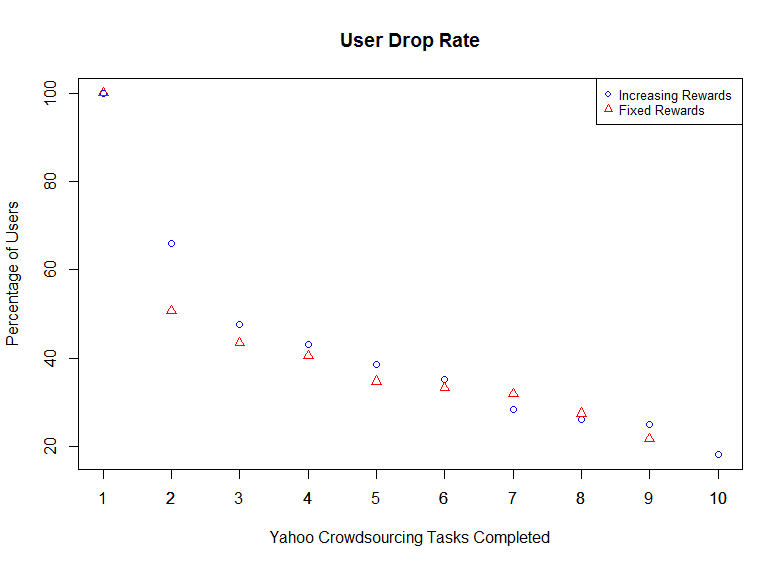
\includegraphics[width=1\linewidth]{images/UserDropRate}
		\caption{Comparision of the user drop rate for the fixed reward scheme and the increasing reward incentive scheme.\label{fig:UserDropRate}}
	\end{center}
\end{figure}

The percentage of rewarded reports during the fixed reward campaign was 64.8\%.
In the increasing reward campaign, the proportion of awarded reports is 62.3\%. Although the difference between the two campaigns is 2.5\%, users on the increasing reward campaign appear to be more predisposed to report without receiving a reward.

Considering all the reports obtained using two different reward schemes, we verify that the reward does not seem to have an impact on the overall emotional reports captured. This effect can be observed in Figure \ref{fig:RewardedvsNonRewarded}.
 
\begin{figure}[htb]
	\begin{center}
		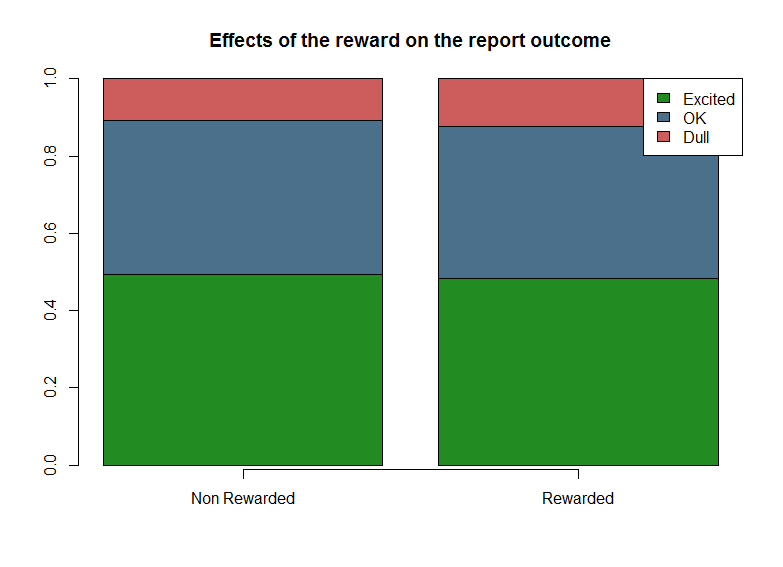
\includegraphics[width=1\linewidth]{images/RewardedvsNonRewarded}
		\caption{The rewards given do not affect the proportion of emotions reported.\label{fig:RewardedvsNonRewarded}}
	\end{center}
\end{figure}

Between reward incentives, the fixed reward scheme also verifies the trend displayed in Figure \ref{fig:RewardedvsNonRewarded}, with very slight differences in the overall emotional reports obtained. On the increasing reward scheme, however, we found that these differences in the emotional reports were more accentuated the rewarded reports displaying a higher ''Dull'' percentage \ref{fig:RewardedsIncreasing}.

\begin{figure}[htb]
	\begin{center}
		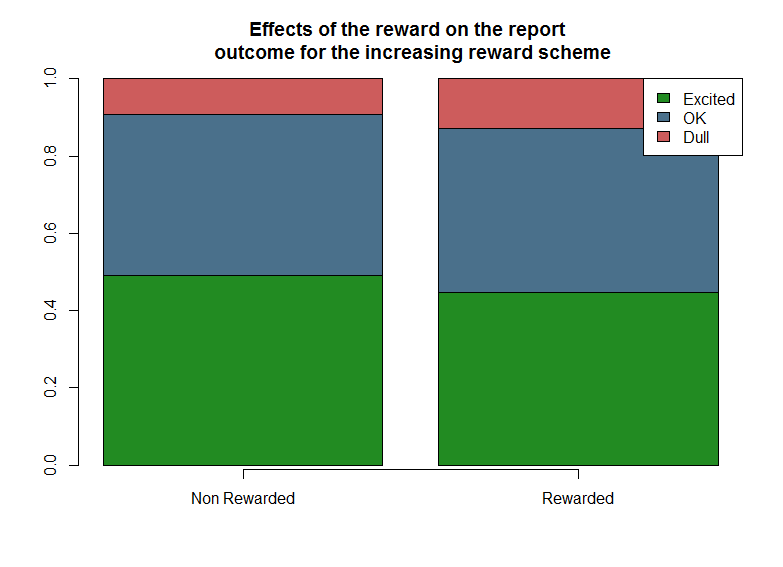
\includegraphics[width=1\linewidth]{images/RewardsIncreasing}
		\caption{Difference between the proportion of  the different emotional states when the report is rewarded or not.\label{fig:RewardedsIncreasing}}
	\end{center}
\end{figure}




\subsection{Genkii Territory}

As location enabled emotional report application, Genkii provides insights on the location of the users and overall mobility.

To capture mobility information we created the concept of ''Genkii Territory'', which we define as the area that spans between the maximum and minimum latitude and the maximum and minimum longitude reached by a player, adjusted for the earth shape, by assuming a sinusoidal projection. This area is an estimate of overall mobility.
It is important to keep in mind that we limited the ability to report consecutively on the same location.

We calculated the "Genkii Territory" for all players that report at least 6 times during both campaigns. There were 65 users that met the requirements set.

Given the fact that the distribution of the areas that we obtained (in $km^2$),
has a great variance, the standard deviation is 19105.4$km^2$, the mean being 4698.00, and the median 81.72. We categorize the players, regarding their mobility according to the bins in Figure \ref{fig:territory}.

Most of the Genkii users who report more often seem to travel daily distances associated with commuting. Either those who stay practically on  the same spot (''House Dwellers'') or those who travel long distances seem to be a minority.

\begin{figure}[htb]
	\begin{center}
		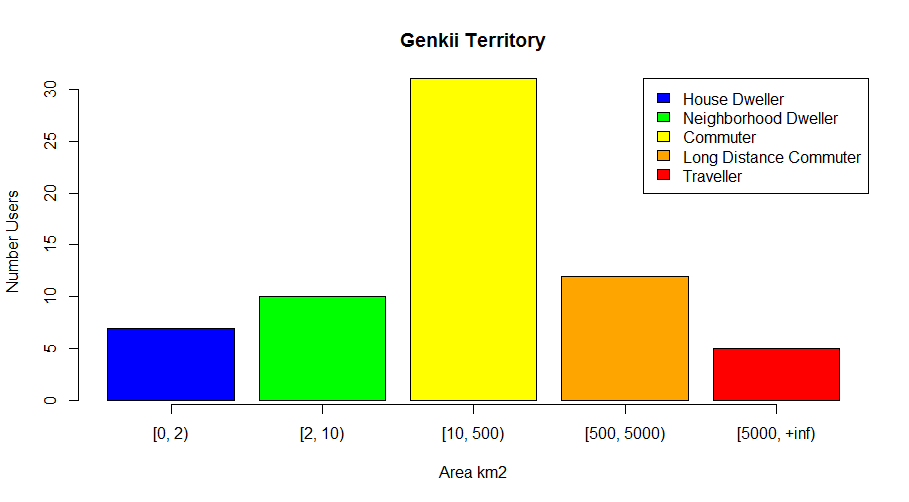
\includegraphics[width=1\linewidth]{images/territory}
		\caption{Genkii territory. Given approximate sizes of cities, we figured 5 naive category ranges to classify our users with regards to their mobility. Those who have a ''Genkii Territory'' that spans for less than 2$km^2$ are called ''House Dwellers''. If they have a territory no larger than 10$km^2$ they are classified as ''Neighborhood Dwellers''. Most of our users have a territory comprised between 10$km^2$ and 500$km^2$ we figured these values could be common for commuters.
			We also define a '''Long Distance Commuter'' category. And for  users which have a ''Genkii Territory'' larger than 5000$km^2$ we supply a ''Traveller'' label. \label{fig:territory}}
	\end{center}
\end{figure}




\subsection{Genkii Distribution}

In order to capture trends over time, we user all the reports collected during both campaigns.
With these results, we seek to understand more about the users who signed with Yahoo Crowdsourcing to provide Genkii reports.

The mean proportion of registered emotions is 49\% of ''Happy reports'', 39\% of ''OK'', and 12\% of ''Sad'' Reports.


In the Figure \ref{fig:genkiioverday} capture the hourly distribution of the reports. We can observe that there seems to be a cyclic pattern during the day, with the lowest amount of reports made at 1, 9, and 17. Culturally it is interesting to verify that these are common commuter times. 
\begin{figure}[htb]
	\begin{center}
		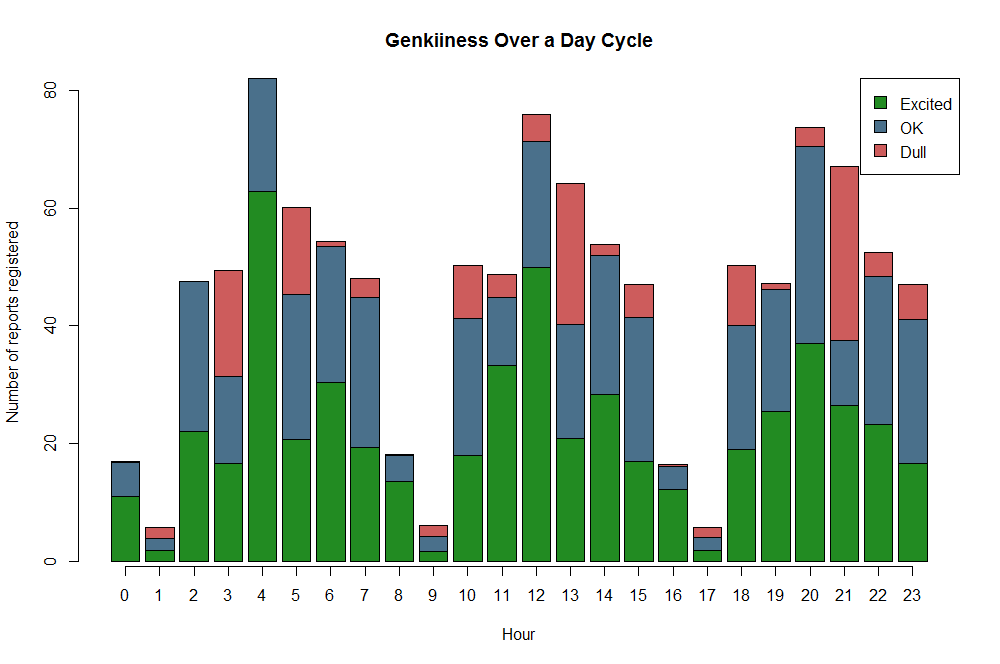
\includegraphics[width=1\linewidth]{images/GenkioverDay}
		\caption{Captured affect reports over a day cycle.\label{fig:genkiioverday}}
	\end{center}
\end{figure}

The fact that we used a total of 1059 reports to construct this visualization seems to help us capture an overall stable group behavior. The daily activity is clearly separated in 8-hour periods.

In contrast, the higher amount of reports seems to be made around 4, 12 and 20. Once again we can hypothesize that around 4 we have a lot of reports from people going out at night. The highest peak of our registered reports happens just before the public transport resumes in the city of Tokyo (around 5). Although the relative proportion of emotions reported seems not to vary much throughout the day, the 3, 4, and 5 seem to be privileged time for expressing emotions. In the 4 a.m. slot, we captured the highest peak of ''Excited'' report. The 3 and 5 a.m. slots see some of the highest proportions of ''Dull'' reports.

Meal times or meal breaks seem also to be privileged by users to make reports. 
We always verify during the hour after the slot with a reports peak there is a rise on general dissatisfaction, which is interesting because the peak report times (4,12, and 20) also represent peaks of the ''Excited'' reports.

These results reinforce that users tend to use the Genkii app as a pastime. 

\subsection{Gestures} 
The accuracy (the gesture predicted by the system being the same as the gesture confirmed), is 85.3\% for the first campaign, and 83.6\% for the second campaign.
The prevalence of left-handed people is similar in both campaigns with 7\% of self-reported left-handed people in the first campaign, and 10\% on the second campaign. Overall the percentage of left-handed people was 9.7\%.

The confirmed accuracy of the gesture predicted was 85\% for the paid reports and 84.3\% for non-rewarded reports. Once again there seems not to be a significant difference between reports that are rewarded and non-rewarded reports.

\section{Discussion}

Despite the inherent advantages of time and reach cost, crowdsourced studies end up forgoing the control over the experimental setting. It is difficult to assure conditions for representative demographics. 
This fine-grained control can be replaced by large numbers in statistical sampling. 


During the first campaign, using fixed rewards, we noticed that 19\% of the users that provide reports ended up providing more reports than the strictly rewarded ones.
This points us to the merit of the application in capturing the users' interest. 
Perhaps the effect of the stable reward experiment made users shift their focus from the reward acquisition to the application. Besides clearly displaying the instructions, and the presence of the timer, Genkii allows the user to explore and play with the application, making reports (as long as successive reports are not made in the same place).

The design decision to use gestures started as a way to promote a mechanical task but ended up providing a playful way to make a Genkii report, which made the non-rewarded reports around 35\% of all reports registered. This points to the fact that Genkii succeeds in keeping the users interested and motivated without inducements. This brings us to an important conclusion: careful design, and toy/game like attributes play an important role in keeping the users engaged. We can go even further in stating that in general we did not verify a difference in the quality of reports because the relative proportions remain practically the same whether the users unlock a reward or not.


From the data captured from the application we were able to categorize the population who enrolled to try the Genkii application and get rewarded by doing so. We found out that most people who joined have a certain degree of mobility, which we associated with commuting. It was also interesting to find that the usage of the application has a periodic behavior, with 8 hour cycles, and there seems to be two mood related changes during those cycles. During the peak reporting times, the ''Excited'' mood proportion tens to increase slightly, while during the following our we experience an increase in ''Dull'' reports.  

In terms of Yahoo Crowdsourcing campaigns we learned that the first three to four days saw the highest number of new users. This may be a limitation in the way the tasks are  promoted in Yahoo Crowdsourcing Japan website, but may be helpful for future campaign design. 

The biggest bridge in terms of user drop rate, as expected is between the first and the second report. Still, when considering user completed tasks, this  drop rate was more accentuated when the initial reward was bigger.





 


\section{Conclusions}



This work provides a case study for anyone interested in pursuing crowd sourced studies with Yahoo Crowdsourcing Japan. First we figure that the amount of rewards did not trigger a very considerable change on the user on-boarding, with both campaigns, even though the increasing reward campaign, which started off with a lower reward managed to attract more users. Analyzing the frequency of one-time reporters, we find that actually the fixed reward campaign attracted more of these users (39) against the 30 users that reported only once.

Our recommendation for future studies is to focus on the first 5 days of the campaign, or split a large campaign into smaller sized ones. The effect of rewards for sequential tasks does not differ drastically when using fixed or increasing rewards. However we noted a smaller user drop rate with the increasing rewards. 

Future developments for Genkii include the application of the knowledge acquired to new areas, such as pain monitoring, disaster response. In either case it would be to our advantage if the application was able to trigger intrinsic motivation in its users.
During the campaigns' time Genkii registered a significant percentage of unpaid reports (around 35\%).  

In this study, we considered only the usage of monetary inducements. There's an extensive literature on gamification, and the usage of other methods to keep the users engaged. Future steps include offering a version with gamification elements, and after a similar user acquisition compare the engagement and drop rates of the study.

The emotional report data collected seems to plausibly explain trends and cultural aspects. One future work could be trying to match and validate this emotional report method with sentiment analysis from Twitter, for example. 



\section{ Acknowledgments}

We thank Daniel Morais for his contribution on the visualization of the Genkii Map website.

\appendix

\section{Fixed Reward Campaign}

\begin{figure}[htb]
	\begin{center}
		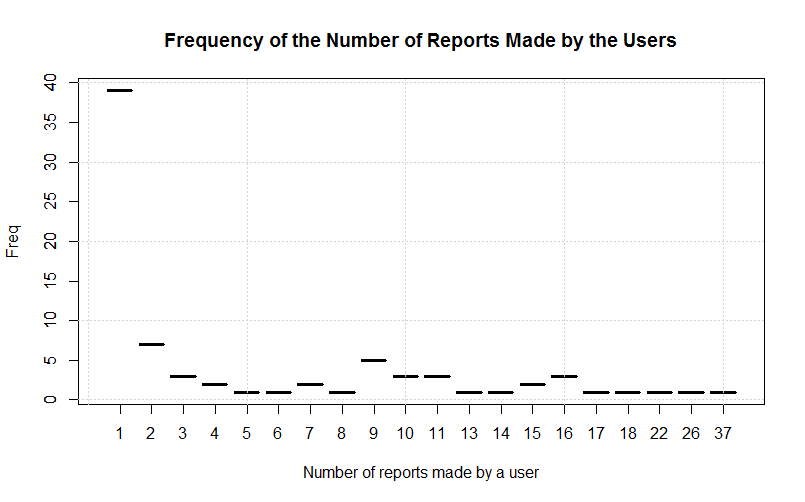
\includegraphics[width=1\linewidth]{images/FrequencyNumberReports_F}
		\caption{Frequency of reports made by users during the fixed reward campaign. As expected, the number of users that made only a single Genkii report (39) stands out. On average each user makes 5.5 reports with a standard deviation of 6.9 reports, the median is 2 reports.\label{fig:freqreports1}}
	\end{center}
\end{figure}

\begin{figure}[htb]
	\begin{center}
		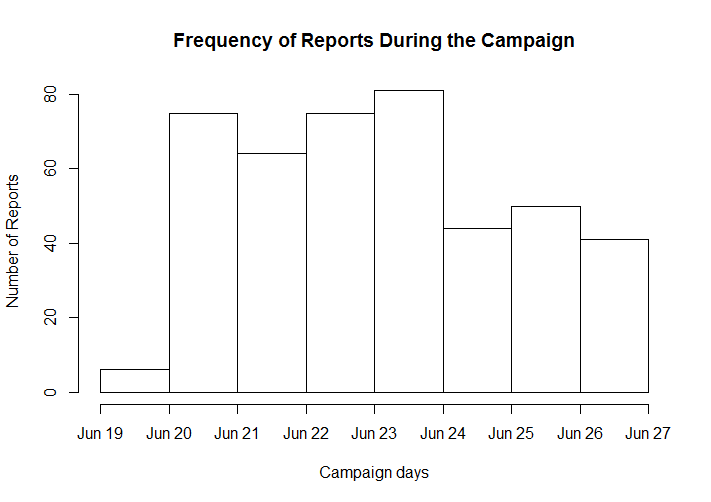
\includegraphics[width=1\linewidth]{images/RPerDay_F}
		\caption{Number of Reports made on each day of the fixed reward campaign.\label{fig:freqreportsperday1}}
	\end{center}
\end{figure}

\begin{figure}[htb]
	\begin{center}
		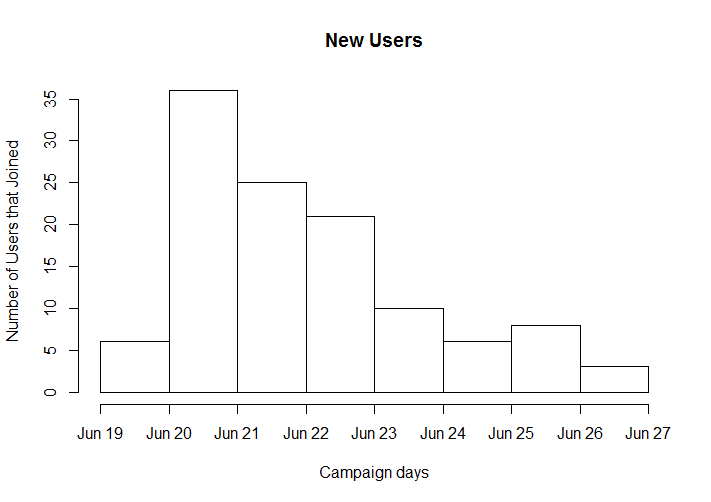
\includegraphics[width=1\linewidth]{images/NewUsers_F}
		\caption{User acquisition throughout the fixed reward campaign.\label{fig:newusers1}}
	\end{center}
\end{figure}

\section{Increasing Reward Campaign}

\begin{figure}[htb]
	\begin{center}
		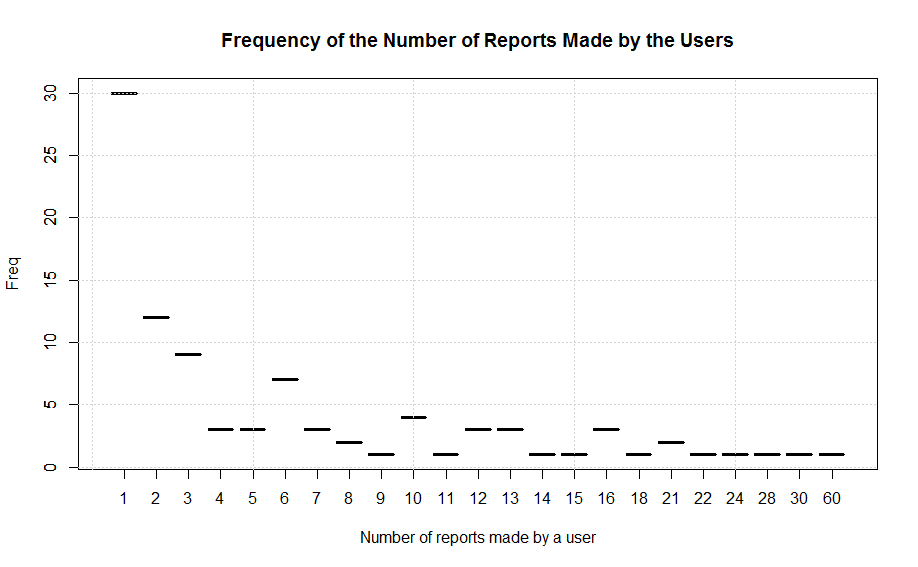
\includegraphics[width=1\linewidth]{images/FrequencyNumberReports_I}
		\caption{Frequency of reports made by users during the increasing reward campaign. As expected, the number of users that made only a single Genkii report (30) stands out. On average each user makes 4.1 reports with a standard deviation of 6.3 reports, the median is 2 reports.\label{fig:freqreports2}}
	\end{center}
\end{figure}

\begin{figure}[htb]
	\begin{center}
		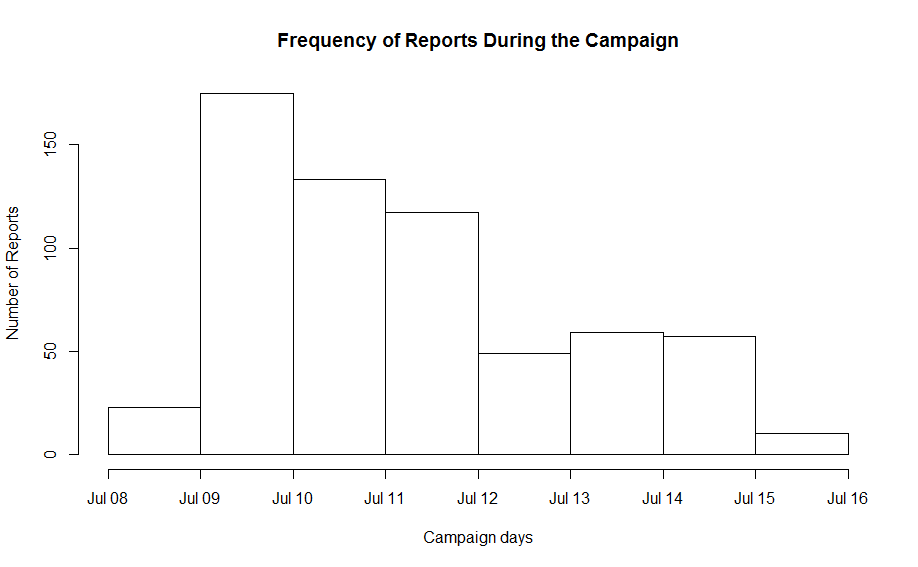
\includegraphics[width=1\linewidth]{images/RPerDay_I}
		\caption{Number of Reports made on each day of the increasing reward campaign .\label{fig:freqreportsperday1}}
	\end{center}
\end{figure}


\begin{figure}[htb]
	\begin{center}
		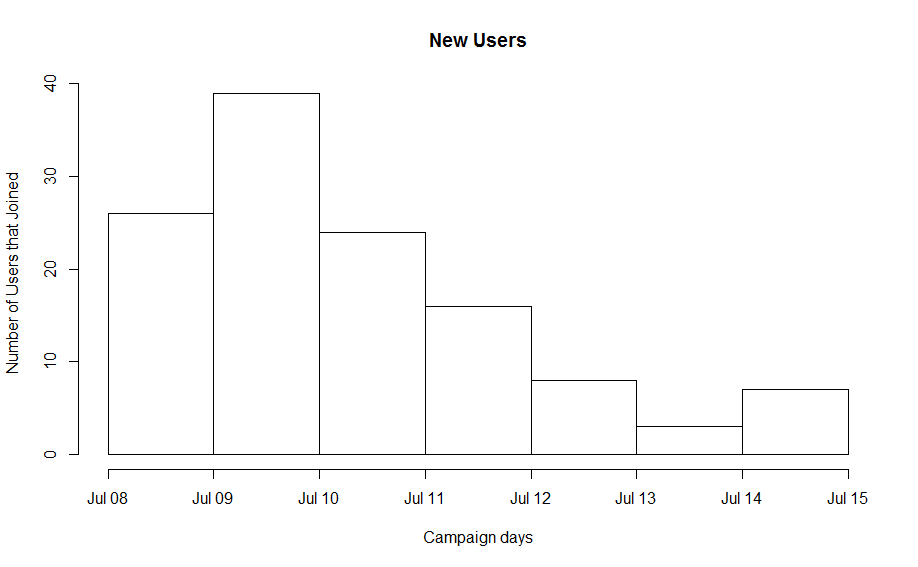
\includegraphics[width=1\linewidth]{images/NewUsers_I}
		\caption{User acquisition throughout the increasing reward campaign.\label{fig:newusers2}}
	\end{center}
\end{figure}


\bibliographystyle{aaai}
\bibliography{genkiarticle}
\end{document}
